\documentclass{beamer}
\usetheme{Madrid}

\usepackage{amsmath}
\usepackage{amssymb}
\usepackage{graphicx}
\usepackage[dvipsnames]{xcolor}
\usepackage[english]{babel}
\usepackage{tikz}
\usepackage{qcircuit}
\usepackage{float}
\usepackage{amsthm}

\usepackage{hyperref}
\hypersetup{
    colorlinks=true,
    linkcolor=blue,
    urlcolor=blue
}

\title{QEC: Classical Errors to the Surface Code}
\author{Daniel Mandragona}
\date{\today}

\begin{document}

\begin{frame}
\titlepage
\end{frame}

\begin{frame}
\frametitle{Table of Contents}
\tableofcontents
\end{frame}

\section{Introduction}

\begin{frame}
\frametitle{Introduction}
\begin{itemize}[<+->]
    \item Quantum computers attempt to solve \emph{certain} computational problems faster than classical computers.
    \item However, QCs are incredibly fragile and susceptible to noise.
    \begin{itemize}
        \item The \emph{basic} theory assumes a closed quantum system.
    \end{itemize}
    \item This leads to a paradox:
\begin{center}
    \textit{How can a completely closed quantum system be \href{https://tenor.com/view/lilo-and-stitch-lilo-stitch-shes-touching-me-im-not-touching-you-gif-14803068}{manipulated} by an observer?}
\end{center}
\end{itemize}
\end{frame}

\begin{frame}
\frametitle{What is Error Correction?}
\begin{itemize}[<+->]
    \item The fundamental idea behind any error correction is to encode information in a \textbf{redundant} way.
    \item Redundancy allows us to detect and correct errors without losing information.
    \item Unfortunately, this is not so straightforward in the quantum setting.
    \begin{itemize}
        \item Non-classical types of errors.
        \item There's no \href{https://tenor.com/view/copy-machine-office-space-printer-fax-kick-gif-5196729}{copying} a quantum state.
    \end{itemize}
\end{itemize}
\vfill
\end{frame}

\section{Classical Error Correction}
{
    \begin{frame}
        \frametitle{Table of Contents}
        \tableofcontents[currentsection]
    \end{frame}
}

\begin{frame}
\frametitle{Classical Error Correction}
\begin{itemize}[<+->]
    \item Bits are physical, not theoretical, and are therefore subject to noise from:
    \begin{itemize}
        \item CPUs overheating
        \item Manufacturing defects
        \item Cosmic rays...
    \end{itemize}
    \item The situation is much better than in the quantum setting, however.
    \begin{itemize}
        \item Error rates are extremely low (e.g., one per billion operations).
        \item Strong error correction methods, like the Hamming code are still in use (e.g., in RAM) today.
    \end{itemize}
\end{itemize}
\end{frame}

\begin{frame}
\frametitle{The Repetition Code: Encoding}
The simplest classical error-correcting code.
\begin{itemize}[<+->]
    \item Goal: Send a single bit (0 or 1) across a noisy channel with a bit-flip probability of $p$.
    \item Encoding: Repeat the bit three times.
    \begin{itemize}
        \item $0 \rightarrow 000$ (Logical 0)
        \item $1 \rightarrow 111$ (Logical 1)
    \end{itemize}
    \item The encoded blocks (000, 111) are called \textbf{codewords}.
\end{itemize}
\end{frame}

\begin{frame}
\frametitle{The Repetition Code: Decoding}
\begin{itemize}[<+->]
    \item Suppose a single bit-flip error occurs during transmission.
    \item Example: We send logical 0 (encoded as 000) and receive 010.
    \item Decoding: The receiver uses a \textbf{majority vote}.
    \item In the case of 010, the majority of bits are 0, so the receiver correctly deduces the original bit was 0.
    \item This simple code can correct any \emph{single} bit-flip error.
\end{itemize}
\end{frame}

\begin{frame}
\frametitle{The Repetition Code: Limitations}
\begin{itemize}[<+->]
    \item The code fails if two or more bits are flipped.
    \item Example: 000 becomes 110. The majority vote would incorrectly decode this as 1.
    % QUESTION FOR AUDIENCE.
    \item What is the probability of failing now?
    \item $\binom{3}{2} p^2(1-p) + \binom{3}{3}p^3 = 3p^2 - 2p^3$
    \item The code is only advantageous if this probability is less than $p$.
    \item We can \textbf{improve} the code by using longer odd-length repetitions.
\end{itemize}
\end{frame}

\section{Linear Codes}
{
    \begin{frame}
        \frametitle{Table of Contents}
        \tableofcontents[currentsection]
    \end{frame}
}

\begin{frame}
\frametitle{Linear Codes}
\begin{itemize}[<+->]
    \item Linear codes are a more sophisticated type of code. Ex. Hamming Code.
    \item A code is \textbf{linear} if the sum of any two codewords is also a codeword.
    \begin{itemize}
        \item "Sum" here means bitwise XOR.
        \item This operation turns the set of bit strings into a vector space modulo 2.
    \end{itemize}
    % QUESTION FOR AUDIENCE.
    % We have that the vector space operation preserves codewords.
    \item Linear codes are described by two matrices:
    \begin{itemize}
        \item \textbf{Generator Matrix ($G$):} Encodes the message.
        \item \textbf{Parity Check Matrix ($H$):} Detects errors.
    \end{itemize}
\end{itemize}
\end{frame}

\begin{frame}
\frametitle{The [7,4] Hamming Code: Encoding}
\begin{itemize}[<+->]
    \item Encodes 4 logical bits into a 7-bit codeword.
    \item The generator matrix $G$ is:
    $$ G = \begin{pmatrix}
    1 & 0 & 0 & 0 & 0 & 1 & 1 \\
    0 & 1 & 0 & 0 & 1 & 0 & 1 \\
    0 & 0 & 1 & 0 & 1 & 1 & 0 \\
    0 & 0 & 0 & 1 & 1 & 1 & 1
    \end{pmatrix} $$
    \item A 4-bit message $m$ is encoded by $c = mG$, what is the bitstring $1011$ encoded as?
    % QUESTION FOR AUDIENCE.
    \item Example: The message $1011$ is encoded as:
    $$ (1,0,1,1)G = (1,0,1,1,0,1,0) $$
\end{itemize}
\end{frame}

\begin{frame}
\frametitle{The [7,4] Hamming Code: Parity Check}
\begin{itemize}[<+->]
    \item The parity check matrix $H$ has the property that for any valid codeword $c$, $Hc^T = 0$.
    \item This means the codewords are in the \textbf{null space} of $H$.
    \item The parity check matrix for the [7,4] Hamming code is:
    $$ H = \begin{pmatrix}
    0 & 0 & 0 & 1 & 1 & 1 & 1 \\
    0 & 1 & 1 & 0 & 0 & 1 & 1 \\
    1 & 0 & 1 & 0 & 1 & 0 & 1
    \end{pmatrix} $$
    \item If the result of $Hc^T$ is non-zero, an error has been detected.
\end{itemize}
\end{frame}

\begin{frame}
\frametitle{The [7,4] Hamming Code: Error Correction}
\begin{itemize}[<+->]
    \item If a codeword $c$ is sent and an error $e$ occurs, the received vector is $r = c + e$.
    \item To find the error, we compute the \textbf{syndrome}:
    $$ s = Hr^T = H(c+e)^T = Hc^T + He^T = He^T $$
    \item The syndrome depends only on the error, not the original codeword!
    \item Now, assume $e$ is a single-bit error, so its a vector with $0$'s everywhere except one place.
    % AUDIENCE QUESTION
    \item What does the syndrome end up being then?
    \item For a single-bit error at position $i$, the syndrome $s$ will be equal to the $i$-th column of $H$.
    \item This allows us to identify and correct the single-bit error.
\end{itemize}
\end{frame}

\begin{frame}
\frametitle{Hamming Distance and Limitations}
\begin{itemize}[<+->]
    \item The \textbf{Hamming distance} is the number of bits in which two codewords differ.
    \item For the repetition code (000, 111), the distance is 3.
    \item For the [7,4] Hamming code, the distance is also 3.
    \item A code with distance $d$ can:
    \begin{itemize}
        \item Detect up to $d-1$ errors.
        \item Correct up to $\lfloor \frac{d-1}{2} \rfloor$ errors.
    \end{itemize}
    \item \textbf{Benefit:} More efficient than the repetition code (7 bits for 4 logical bits vs. 3 for 1).
\end{itemize}
\end{frame}

\section{Quantum Error Correction}
{
    \begin{frame}
        \frametitle{Table of Contents}
        \tableofcontents[currentsection]
    \end{frame}
}
\begin{frame}
\frametitle{Why Quantum Error Correction is Harder}
QEC is more complex than classical error correction for several reasons:
\begin{enumerate}
    \item \textbf{More error types:} Beyond bit-flips, qubits can have phase-flips, and a continuous range of other errors.
    \item \textbf{No-Cloning Theorem:} We cannot simply copy a qubit to create redundancy.
    \item \textbf{Measurement is destructive:} Measuring a qubit to check for errors collapses its state, destroying the information we want to protect.
\end{enumerate}
Seems \href{https://www.youtube.com/watch?v=XtllaukM9mc}{difficult}...
\end{frame}

\section{The 3-Qubit Bit-Flip Code}

\begin{frame}
\frametitle{The 3-Qubit Bit-Flip Code: Encoding}
A quantum version of the repetition code to correct bit-flip errors.
\begin{itemize}[<+->]
    \item Goal: Encode a single logical qubit:
    $$|\psi\rangle = \alpha|0\rangle + \beta|1\rangle$$
    \item Encoding: Create an entangled three-qubit state:
    $$|\psi_L\rangle = \alpha|000\rangle + \beta|111\rangle$$
    \item This is NOT cloning. The No-Cloning Theorem forbids making independent copies like:
    $$ |\psi_{\text{copied}}\rangle = (\alpha|0\rangle + \beta|1\rangle)^{\otimes 3}$$
\end{itemize}
\end{frame}

\begin{frame}
\frametitle{The CNOT Gate}
\begin{itemize}[<+->]
    \item The Controlled-NOT (CNOT) gate is a two-qubit gate that flips the target qubit if the control qubit is $|1\rangle$.
    \item Matrix representation:
    $$ CNOT = \begin{pmatrix}
        1 & 0 & 0 & 0 \\ 
        0 & 1 & 0 & 0 \\ 
        0 & 0 & 0 & 1 \\ 
        0 & 0 & 1 & 0 \end{pmatrix} $$
        acting on bases: $|00\rangle,|01\rangle,|10\rangle,|11\rangle$.
    \item Circuit diagram:
\end{itemize}
\begin{figure}[H]
\centering
\makebox[\textwidth][c]{
\Qcircuit @C=1em @R=.7em {
\lstick{\text{control}} & \ctrl{1} & \qw \\
\lstick{\text{target}} & \targ & \qw
}
}
\end{figure}
\end{frame}

\begin{frame}
\frametitle{Encoding Circuit for 3 Qubit Bit-Flip Code}
We use two CNOT gates to create the logical state $|\psi_L\rangle$:
\begin{columns}
\column{0.5\textwidth}
\begin{figure}[H]
\centering
\makebox[\textwidth][c]{
\Qcircuit @C=1em @R=.7em {
\lstick{|\psi \rangle} & \ctrl{1} & \ctrl{2} & \qw \\
\lstick{|0 \rangle} & \targ & \qw & \qw \\
\lstick{|0 \rangle} & \qw & \targ & \qw
}
}
\end{figure}
\column{0.5\textwidth}
$$\begin{pmatrix}
        1 & 0 & 0 & 0 \\ 
        0 & 1 & 0 & 0 \\ 
        0 & 0 & 0 & 1 \\ 
        0 & 0 & 1 & 0
    \end{pmatrix}
    \begin{pmatrix}
        \alpha \\
        0 \\
        \beta \\
        0
    \end{pmatrix}$$
\end{columns}
\begin{example}[Creating $|\psi_L\rangle$]
The circuit transforms the initial state $|\psi\rangle|0\rangle|0\rangle$:
\begin{align*}
    |\psi_{initial}\rangle &= (\alpha|0\rangle + \beta|1\rangle)|00\rangle = \alpha|000\rangle + \beta|100\rangle \\
    \xrightarrow{CNOT_{12}}&\,\, \alpha|000\rangle + \beta|110\rangle \\
    \xrightarrow{CNOT_{13}}&\,\, \alpha|000\rangle + \beta|111\rangle = |\psi_L\rangle
\end{align*}
\end{example}
\end{frame}

\begin{frame}
\frametitle{Quantum Errors: Pauli Operators}
\begin{itemize}[<+->]
    \item A \textbf{bit-flip error} is represented by the Pauli $X$ operator:
    $$ X = \begin{pmatrix} 0 & 1 \\ 1 & 0 \end{pmatrix} $$
    It flips the state: $X|0\rangle = |1\rangle$ and $X|1\rangle = |0\rangle$.
    \item A \textbf{phase-flip error} is represented by the Pauli $Z$ operator:
    $$ Z = \begin{pmatrix} 1 & 0 \\ 0 & -1 \end{pmatrix} $$
    It flips the phase: $Z|0\rangle = |0\rangle$ and $Z|1\rangle = -|1\rangle$.
    \item We even have a third error represented by the Pauli $Y$ operator:
    $$ Y = \begin{pmatrix} 0 & -i \\ i & 0 \end{pmatrix} $$
    \item These operators satisfy the property: $XYZ = i$, so $Y = iXZ$, and are \emph{their own inverses}.
\end{itemize}
\end{frame}

\begin{frame}
\frametitle{Detecting Errors Without Measurement}
How do we detect an error like $X_1$ on $|\psi_L\rangle$ without collapsing the state?
\begin{itemize}[<+->]
    \item We can't measure the qubits directly.
    \item Solution: Use \textbf{stabilizer} measurements. These are like the parity checks from classic error correction.
    \item For the bit-flip code, the stabilizers are $Z_1Z_2$ and $Z_2Z_3$.
    \item We measure a \emph{joint} property of these operators, not the individual qubits. We collapse the \emph{correlation}, not the individual states.
\end{itemize}
\end{frame}

\begin{frame}
\frametitle{Measurement Intuition}
\begin{itemize}[<+->]
    \item Quantum measurement is about defining an observable property of your system.
    \item The property is \emph{observable} meaning that the values this property can hold are real-valued.
    \item Measuring an observable is then about projecting your system onto the system states associated to each of these values.
    \item These observables in QC are matrices which can be decomposed into a set of projection matrices:
    $$\mathcal{O} = \lambda_1 P_1 + \dots + \lambda_k P_k$$ 
    \item Your quantum state can then be \emph{written} w.r.t. the bases of each one of the Projection Matrices.
    \item Measurement collapses the state onto the eigenspace associated with the measured eigenvalue.
    The probability of collapsing to a specific eigenspace $k$ is $p(k) = \| P_k |\psi\rangle \|^2$.".
\end{itemize}
\end{frame}

\begin{frame}
\frametitle{Stabilizer Measurement Circuit}
\begin{itemize}[<+->]
\item So how would we \emph{measure} a $Z_1Z_2$ observable?
\item This circuit measures the $Z_1Z_2$ stabilizer using an ancilla qubit.
\begin{figure}[h!]
\centering
\makebox[\textwidth][c]{
\Qcircuit @C=1em @R=.7em {
\lstick{\text{qubit 1}} & \qw & \gate{Z} & \qw & \qw & \qw \\
\lstick{\text{qubit 2}} & \qw & \qw & \gate{Z} & \qw & \qw \\
\lstick{\text{ancilla}} & \gate{H} & \ctrl{-2} & \ctrl{-1} & \gate{H} & \meter
}
}
\end{figure}
\item The measurement outcome of the ancilla tells us the eigenvalue of $Z_1Z_2$.
\end{itemize}
\end{frame}

\begin{frame}
\frametitle{State Evolution: No Error}
\begin{itemize}[<+->]
    \item Note: $|\psi_L\rangle = \alpha|000\rangle + \beta|111\rangle$ is a $+1$ eigenstate of $Z_1Z_2$.
    \item Initial state: $|\psi_L\rangle|0\rangle_a = (\alpha|000\rangle + \beta|111\rangle)|0\rangle_a$.
    \item \textbf{1. Hadamard on ancilla:}
    $$ |\psi_L\rangle\frac{1}{\sqrt{2}}(|0\rangle_a + |1\rangle_a) = |\psi_L\rangle\otimes|+\rangle$$
    \item \textbf{2. Controlled-Z gates:} Since $Z_1Z_2|\psi_L\rangle = |\psi_L\rangle$, the state is unchanged.
    $$ |\psi_L\rangle \otimes |+\rangle_a $$
    \item \textbf{3. Hadamard on ancilla:}
    $$ |\psi_L\rangle \otimes H|+\rangle_a = |\psi_L\rangle|0\rangle_a $$
    \item \textbf{4. Measure ancilla:} Result is $\mathbf{0}$ with certainty. No error detected.
\end{itemize}
\end{frame}

\begin{frame}
\frametitle{State Evolution: With an $X_1$ Error}
\begin{itemize}[<+->]
    \item Note: $|\psi_L\rangle = \alpha|100\rangle + \beta|011\rangle$ is a $-1$ eigenstate of $Z_1Z_2$.
    \item Initial state: $|\psi_{err}\rangle = X_1|\psi_L\rangle = \alpha|100\rangle + \beta|011\rangle$.
    \item \textbf{1. Hadamard on ancilla:}
    $$ |\psi_{err}\rangle\frac{1}{\sqrt{2}}(|0\rangle_a + |1\rangle_a) = |\psi_{err}\rangle\otimes|+\rangle$$
    \item \textbf{2. Controlled-Z gates:} Since $Z_1Z_2|\psi_{err}\rangle = -|\psi_{err}\rangle$, the state becomes:
    \begin{align*} \text{$C_a$-$Z_1Z_2$} \bigl(|\psi_{err}\rangle\frac{1}{\sqrt{2}}(|0\rangle_a + |1\rangle_a)\bigl) &= \frac{1}{\sqrt{2}}(|\psi_{err}\rangle|0\rangle_a - |\psi_{err}\rangle |1\rangle_a) \\
        & = |\psi_{err}\rangle \otimes |-\rangle_a
    \end{align*}
    \item \textbf{3. Hadamard on ancilla:}
    $$ |\psi_{err}\rangle \otimes H|-\rangle_a = |\psi_{err}\rangle|1\rangle_a $$
    \item \textbf{4. Measure ancilla:} Result is $\mathbf{1}$ with certainty. Error detected!
\end{itemize}
\end{frame}

% \begin{frame}
% \frametitle{Phase Kickback: How it Works}
% The error information is transferred to the ancilla via \textbf{phase kickback}.
% \begin{itemize}
%     \item The data qubits are in an eigenstate of the stabilizer $S = Z_1Z_2$ with eigenvalue $\lambda = \pm 1$.
%     \item The ancilla is in a superposition state $|+\rangle$.
%     \item The controlled operation $C-S$ kicks the phase back to the ancilla:
%     $$ |\psi\rangle |+\rangle_a \xrightarrow{C-S} |\psi\rangle \left(\frac{|0\rangle_a + \lambda |1\rangle_a}{\sqrt{2}}\right) $$
%     \item The data state $|\psi\rangle$ is undisturbed. The eigenvalue $\lambda$ is now in the ancilla's phase.
%     \item Measuring the ancilla in the X-basis reveals $\lambda$.
% \end{itemize}
% \end{frame}

\begin{frame}
\frametitle{Error Syndromes}
The measurement outcomes of the stabilizers form the \textbf{error syndrome}.
\begin{itemize}[<+->]
    \item The logical state $|\psi_L\rangle$ is a $+1$ eigenstate of both $Z_1Z_2$ and $Z_2Z_3$.
    \item An error like $X_1$ changes the eigenvalues:
    \begin{align*}
        Z_1Z_2(X_1|\psi_L\rangle) &= -1(X_1|\psi_L\rangle) \\
        Z_2Z_3(X_1|\psi_L\rangle) &= +1(X_1|\psi_L\rangle)
    \end{align*}
    \item The syndrome identifies the error:
    \begin{itemize}
        \item Syndrome (-1, +1) $\implies$ $X_1$ error
        \item Syndrome (+1, -1) $\implies$ $X_3$ error
        \item Syndrome (-1, -1) $\implies$ $X_2$ error
        \item Syndrome (+1, +1) $\implies$ No error
    \end{itemize}
    \item Once identified, we apply the same operator again to correct it.
\end{itemize}
\end{frame}


\section{The 3-Qubit Phase-Flip Code}
{
    \begin{frame}
        \frametitle{Table of Contents}
        \tableofcontents[currentsection]
    \end{frame}
}

\begin{frame}
\frametitle{The 3-Qubit Phase-Flip Code}
\begin{itemize}[<+->]
    \item Now that we can correct bit-flip errors, we must handle \textbf{phase-flips} ($Z$ errors).
    $$\alpha|0\rangle + \beta|1\rangle \Leftrightarrow \alpha|0\rangle - \beta|1\rangle$$
    \item A phase-flip becomes a "bit-flip" in the Hadamard basis $|+\rangle, |-\rangle$.
    \begin{itemize}
        \item $Z|+\rangle = |-\rangle$ and $Z|-\rangle = |+\rangle$.
    \end{itemize}
    \item We use a similar code to the bit-flip code, but in a different basis.
    \item \textbf{Encoding}:
    $$|\psi_L\rangle = \alpha|+++\rangle + \beta|---\rangle$$
    where $|+\rangle = \frac{1}{\sqrt{2}}(|0\rangle + |1\rangle)$ and $|-\rangle = \frac{1}{\sqrt{2}}(|0\rangle - |1\rangle)$.
\end{itemize}
\end{frame}

\begin{frame}
\frametitle{Phase-Flip Code: Encoding Circuit}
The encoding circuit uses Hadamards to change basis.
\begin{figure}[H]
\centering
\makebox[\textwidth][c]{
\Qcircuit @C=1em @R=.7em {
\lstick{|\psi\rangle} & \ctrl{1} & \ctrl{2} & \gate{H} & \qw \\
\lstick{|0\rangle} & \targ & \qw & \gate{H} & \qw \\
\lstick{|0\rangle} & \qw & \targ & \gate{H} & \qw
}
}
\end{figure}
\begin{itemize}
    \item The stabilizers for this code are $X_1X_2$ and $X_2X_3$.
    \item A $Z$ error on one qubit will flip the sign of one or both stabilizer measurements, revealing the error.
\end{itemize}
\end{frame}

\begin{frame}
\frametitle{Phase-Flip Code: Syndrome Measurement}
The syndrome measurement circuit is analogous to the bit-flip code's, but with controlled-X gates.
\begin{figure}[H]
\centering
\makebox[\textwidth][c]{
\Qcircuit @C=1em @R=.7em {
\lstick{\text{qubit 1}} &\qw & \qw & \gate{X} & \qw & \qw & \qw & \qw & \qw \\
\lstick{\text{qubit 2}} &\qw & \qw & \qw & \gate{X} & \gate{X} & \qw & \qw & \qw \\
\lstick{\text{qubit 3}} &\qw & \qw & \qw & \qw & \qw & \gate{X} & \qw & \qw \\
\lstick{\text{ancilla 1}} & \gate{H} & \qw & \ctrl{-3} & \ctrl{-2} & \qw & \qw & \gate{H} & \meter \\
\lstick{\text{ancilla 2}} & \gate{H} & \qw & \qw & \qw & \ctrl{-3} & \ctrl{-2} & \gate{H} & \meter
}
}
\caption{Circuit for measuring errors in the phase-flip code.}
\end{figure}
\end{frame}

\section{The Shor Code}

\begin{frame}
\frametitle{The Shor Code: The First QEC Code}
\begin{itemize}[<+->]
    \item The first quantum error correcting code, created by Peter Shor in 1995.
    \item It combines the bit-flip and phase-flip codes to correct any arbitrary single-qubit error.
    \item It encodes 1 logical qubit into 9 physical qubits.
\end{itemize}
\end{frame}

\begin{frame}
\frametitle{Shor Code: Encoding}
Encoding is a two-step concatenation:
\begin{enumerate}
    \item \textbf{Outer Code (Phase-Flip):} The logical qubit is first encoded to 3 qubits.
    \begin{itemize}
        \item $\alpha|0\rangle + \beta|1\rangle \rightarrow \alpha|+++\rangle + \beta|---\rangle$
    \end{itemize}
    \item \textbf{Inner Code (Bit-Flip):} Each of these 3 qubits is then encoded into 3 more qubits.
    \begin{itemize}
        \item $|+\rangle \rightarrow \frac{1}{\sqrt{2}}(|000\rangle+|111\rangle)$
        \item $|-\rangle \rightarrow \frac{1}{\sqrt{2}}(|000\rangle-|111\rangle)$
    \end{itemize}
\end{enumerate}
This results in a 9-qubit state:
\begin{align*}
    |0_L\rangle &\to \frac{1}{2\sqrt{2}}(|000\rangle+|111\rangle)\otimes(|000\rangle+|111\rangle)\otimes(|000\rangle+|111\rangle) \\
    |1_L\rangle &\to \frac{1}{2\sqrt{2}}(|000\rangle-|111\rangle)\otimes(|000\rangle-|111\rangle)\otimes(|000\rangle-|111\rangle)
\end{align*}
\end{frame}

\begin{frame}
\frametitle{How Shor Code Corrects Bit-Flips}
The 9 qubits are grouped into three blocks of three. Each block is a bit-flip code.
\begin{itemize}[<+->]
    \item If a single bit-flip error occurs on any qubit (e.g., $q_1$), it happens within one block.
    \item The inner code's stabilizers for that block ($Z_1Z_2, Z_2Z_3$) will detect the error.
    \item The syndrome identifies the errored qubit.
    \item We apply another $X$ gate to that qubit to correct it.
    \item This works for any single bit-flip on any of the 9 qubits.
\end{itemize}
\end{frame}

\begin{frame}
\frametitle{How Shor Code Corrects Phase-Flips}
The outer code is a phase-flip code, where each "qubit" is one of the 3-qubit blocks.
\begin{itemize}[<+->]
    \item A single phase-flip error ($Z$) on one physical qubit is equivalent to a logical phase-flip on its block.
    \item Example: $Z_1$ on $\frac{1}{\sqrt{2}}(|000\rangle+|111\rangle)$ gives $\frac{1}{\sqrt{2}}(|000\rangle-|111\rangle)$.
    \item The outer code's stabilizers detect which block has the phase error.
    \item These stabilizers are logical $X$ operators of the inner codes, e.g., $(X_1X_2X_3)(X_4X_5X_6)$.
    \item Once the block is identified, we apply a $Z$ gate to one of its qubits to correct the error.
\end{itemize}
\end{frame}

\begin{frame}
\frametitle{Shor Code: $Y$ Errors}
\begin{itemize}[<+->]
    \item The Shor code can correct both bit-flip ($X$) and phase-flip ($Z$) errors on any single qubit.
    \item A $Y$ error ($=iXZ$) is a rotated combination of $X$ and $Z$.
    \item How can we deal with this $i$ factor?
    \item In fact, errors are always a linear combination of the pauli bases.
    \item How can we deal with a \emph{continuous} range of errors?
\end{itemize}
\end{frame}


\section{Correcting Any Quantum Error}
{
    \begin{frame}
        \frametitle{Table of Contents}
        \tableofcontents[currentsection]
    \end{frame}
}

\begin{frame}
\frametitle{Errors as a Superposition}
\begin{itemize}[<+->]
    \item Any arbitrary single-qubit error, represented by a matrix $E$, can be expressed as a linear combination of Pauli matrices:
    $$ E = c_i I + c_x X + c_y Y + c_z Z $$
    \item What happens when an error $E$ acts on a logical state $|\psi_L\rangle$?
    \item The result is a superposition of the original state and the three Pauli errors acting on it:
    $$ E|\psi_L\rangle = c_i I|\psi_L\rangle + c_x X|\psi_L\rangle + c_y Y|\psi_L\rangle + c_z Z|\psi_L\rangle $$
\end{itemize}
\end{frame}

\begin{frame}
\frametitle{Error Discretization via Measurement}
\begin{itemize}[<+->]
    \item When we measure the stabilizers of the code, the state collapses.
    \begin{itemize}
        \item Collapses $\implies$ The $c$ goes away.
        \item Ex: Collapses to $X$ with probability $|c_x|^2$.
    \end{itemize}
    \item This has the effect of \textbf{discretizing} the error. The state snaps to one of four possibilities:
    \begin{itemize}
        \item No error ($I$)
        \item An $X$ error
        % QUESTION FOR AUDIENCE
        % Where does the i factor go?
        \item A $Z$ error
        \item A $Y$ error
    \end{itemize}
\end{itemize}
\pause
\begin{alertblock}{Requirements for Error Discretization}
    \begin{itemize}
        \item Stabilizers must be able to actually detect the Pauli error basis.
        \item \emph{Simultaneous} stabilizer measurements require their stabilizers to \textbf{commute}.
    \end{itemize}
\end{alertblock}
\end{frame}

\begin{frame}
\frametitle{Summarizing Discretization}
\begin{itemize}[<+->]
    \item The syndrome measurements tells us \textit{which} discrete Pauli error occurred and \textit{where}.
    \item Shor stabilizers commute with each other (so that we can measure them simultaneously).
    \begin{itemize}
        \item Ex: Outer stabilizers like: $(X_1X_2X_3)(X_4X_5X_6)$ commute with inner stabilizers $Z_1Z_2$ and $Z_2Z_3$.
    \end{itemize}
    \item Once the error is identified, we simply apply the same operator again to reverse it (since Pauli operators are their own inverse).
    \item \textbf{Conclusion:} By correcting only the discrete Pauli errors, we can correct any arbitrary single-qubit error.
\end{itemize}
\end{frame}


\section{The Stabilizer Formalism}
{
    \begin{frame}
        \frametitle{Table of Contents}
        \tableofcontents[currentsection]
    \end{frame}
}

\begin{frame}
\frametitle{The Stabilizer Formalism}
\begin{itemize}[<+->]
    \item A powerful \href{https://tenor.com/view/chicken-isolate-shake-gif-16060042}{framework} for constructing and understanding QEC codes.
    \item The bit-flip, phase-flip, and Shor codes are all examples of \textbf{stabilizer codes}.
    \item A stabilizer code is defined by a set of commuting Pauli operators $\{S_i\}$ called the \textbf{stabilizers}.
    \item The full set, $\mathcal{S}$, is a commutative group that is \emph{generated} by a smaller set of \emph{independent} stabilizers.
    \item Start with $G = \{g_1,g_2,\dots,g_n\}$ then: $$\mathcal{S} = \{S_i | S_i = \prod_{g_i \in A} g_i, A \subset G\}$$    
    \item Caution: We can't include $-I$ in $\mathcal{S}$ (next slide will explain why).
\end{itemize}
\end{frame}

\begin{frame}
\frametitle{How Stabilizer Codes Work}
\begin{itemize}[<+->]
    \item The \textbf{codespace} is the subspace of states $|\psi\rangle$ that are left unchanged (+1 eigenvalue) by all stabilizers:
    $$S_i|\psi\rangle = +1|\psi\rangle \quad \text{for all } S_i \in \mathcal{S}$$
    \item Made from Pauli operators so the values that each property can be is in $\{+1, -1\}$.
    \item Each stabilizer generator splits the quantum space in half.
    \begin{itemize}
        % QUESTION FOR AUDIENCE
        % Why does this prove the halving?
        \item Trace of Pauli operators is 0. Hint: Trace is the sum of eigenvalues (including repetition). 
    \end{itemize} 
    \item An error $E$ occurs. The state $E|\psi\rangle$ may no longer be a $+1$ eigenstate of some stabilizers.
    \item We measure all stabilizer generators to get the \textbf{error syndromes}.
\end{itemize}
\end{frame}

\section{The 5-Qubit Code}
{
    \begin{frame}
        \frametitle{Table of Contents}
        \tableofcontents[currentsection]
    \end{frame}
}

\begin{frame}
\frametitle{The 5-Qubit Code: The Smallest Perfect Code}
\begin{itemize}[<+->]
    \item The most \emph{efficient} code possible for protecting 1 logical qubit from any single-qubit error.
    \item It encodes 1 logical qubit into 5 physical qubits.
    \item It satisfies the \textbf{Quantum Hamming Bound} where $n$ is physical qubits and $k$ is logical qubits:
    % QUESTION FOR AUDIENCE
    % What are the values of the left and RHS?
    \begin{align*}
        \text{\# of syndromes} &\geq \text{\# of important configurations} \\
        2^{n-k} &\geq 1 + 3n
    \end{align*}
    \item For $n=5, k=1$:
    $$ 2^{5-1} = 16 \geq 1 + 3(5) = 16 $$
    \item Caveat: This requires a non-degenerate quantum code, meaning that every correctable error has a unique syndrome. 
\end{itemize}
\end{frame}

\begin{frame}
\frametitle{5-Qubit Code: Stabilizers}
\begin{itemize}[<+->]
    \item We need $n-k = 4$ independent and commuting stabilizers to define a two dimensional codespace for a logical qubit.
    \item The four commuting stabilizer generators are:
    \begin{align*}
        S_1 &= X \otimes Z \otimes Z \otimes X \otimes I \\
        S_2 &= I \otimes X \otimes Z \otimes Z \otimes X \\
        S_3 &= X \otimes I \otimes X \otimes Z \otimes Z \\
        S_4 &= Z \otimes X \otimes I \otimes X \otimes Z
    \end{align*}
\end{itemize}
\end{frame}

\begin{frame}
\frametitle{5-Qubit Code: Logical Operators}
\begin{itemize}[<+->]
    \item Logical operators act on the encoded qubit without leaving the codespace.
    \item They must commute with all stabilizers but not be in the stabilizer group themselves.
    \item They must anti-commute with each other ($\bar{X}\bar{Z} = -\bar{Z}\bar{X}$), forming a valid logical qubit.
    \begin{itemize}
        \item This gives us the uncertainty principle from within this protected subspace, and enables us to rebuild the Pauli algebra/bloch sphere.
    \end{itemize}
    \item The logical operators for the 5-qubit code are:
    \begin{align*}
        \bar{X} &= X \otimes X \otimes X \otimes X \otimes X \\
        \bar{Z} &= Z \otimes Z \otimes Z \otimes Z \otimes Z
    \end{align*}
\end{itemize}
\end{frame}

\begin{frame}
\frametitle{5-Qubit Code Summary}
\begin{itemize}[<+->]
    \item A code is often described by $[[n,k,d]]$:
    \begin{itemize}
        \item $n$: number of physical qubits
        \item $k$: number of logical qubits
        \item $d$: \textbf{code distance}
    \end{itemize}
    \item The code distance $d$ is the minimum weight (single qubit Pauli operations) of a non-trivial logical operator.
    \item For the 5-qubit code, $d=3$. This means it can correct $t = \lfloor \frac{3-1}{2} \rfloor = 1$ error.
\end{itemize}
\end{frame}

\section{The Surface Code}
{
    \begin{frame}
        \frametitle{Table of Contents}
        \tableofcontents[currentsection]
    \end{frame}
}

\begin{frame}
\frametitle{The Surface Code: Overview}
\begin{itemize}[<+->]
    \item A QEC code that is a realistic prospect for building a fault-tolerant quantum computer.
    \item \textbf{Key Features}:
    \begin{itemize}
        \item Only requires nearest-neighbor interactions between qubits on a 2D grid.
        \item Has a high \textbf{threshold error rate}, tolerating more noise.
    \end{itemize}
    \item It is a \textbf{\href{https://tenor.com/view/cup-torus-hole-tea-coffee-gif-26670784}{topological} code}: its properties are protected by the global structure of the system.
\end{itemize}
\end{frame}

\begin{frame}
\frametitle{Surface Code: The Lattice}
\begin{itemize}[<+->]
    \item Data qubits reside on the \textbf{edges} of a 2D lattice.
    \item Stabilizers are defined based on the vertices and faces (plaquettes) of the lattice.
\end{itemize}
\begin{figure}
\centering
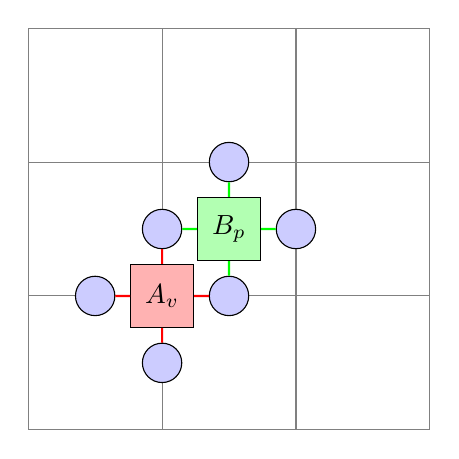
\begin{tikzpicture}[scale=1.7]
    \tikzstyle{dataq} = [circle, draw, fill=blue!20, inner sep=0pt, minimum size=5mm]
    \tikzstyle{vertexop} = [rectangle, draw, fill=red!30, inner sep=0pt, minimum size=8mm]
    \tikzstyle{plaqop} = [rectangle, draw, fill=green!30, inner sep=0pt, minimum size=8mm]
    \draw[gray, thin] (0,0) grid (3,3);
    \node[dataq] (q01v) at (1, 0.5) {}; \node[dataq] (q10h) at (0.5, 1) {};
    \node[dataq] (q11v) at (1, 1.5) {}; \node[dataq] (q11h) at (1.5, 1) {};
    \node[dataq] (q12h) at (1.5, 2) {}; \node[dataq] (q21v) at (2, 1.5) {};
    \node[vertexop] (A11) at (1,1) {$A_v$}; \node[plaqop] (B11) at (1.5,1.5) {$B_p$};
    \draw[red, thick] (q01v) -- (A11); \draw[red, thick] (q10h) -- (A11);
    \draw[red, thick] (q11v) -- (A11); \draw[red, thick] (q11h) -- (A11);
    \draw[green, thick] (q11v) -- (B11); \draw[green, thick] (q11h) -- (B11);
    \draw[green, thick] (q12h) -- (B11); \draw[green, thick] (q21v) -- (B11);
\end{tikzpicture}
\end{figure}
\end{frame}

\begin{frame}
\frametitle{Surface Code: The Stabilizers}
\begin{columns}
    \column{0.5\textwidth}
    \begin{itemize}
        \item \textbf{Star operators ($A_v$):} Product of $X$ on qubits meeting at a vertex $v$.
        $$ A_v = \bigotimes_{i \in \text{star}(v)} X_i $$
        \item \textbf{Plaquette operators ($B_p$):} Product of $Z$ on qubits bounding a face $p$.
        $$ B_p = \bigotimes_{i \in \text{boundary}(p)} Z_i $$
    \end{itemize}
    \column{0.5\textwidth}
    \begin{figure}
    \centering
    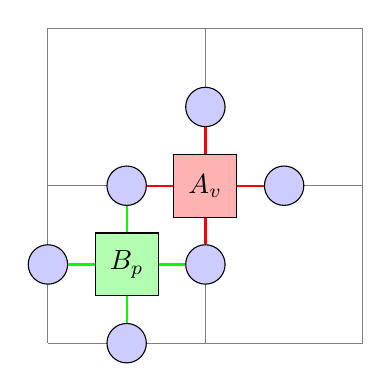
\begin{tikzpicture}[scale=2.0]
        \tikzstyle{dataq} = [circle, draw, fill=blue!20, inner sep=0pt, minimum size=5mm]
        \tikzstyle{vertexop} = [rectangle, draw, fill=red!30, inner sep=0pt, minimum size=8mm]
        \tikzstyle{plaqop} = [rectangle, draw, fill=green!30, inner sep=0pt, minimum size=8mm]
        \draw[gray, thin] (0,0) grid (2,2);
        \node[dataq] (q1) at (0.5, 1) {};
        \node[dataq] (q2) at (1.5, 1) {};
        \node[dataq] (q3) at (1, 0.5) {};
        \node[dataq] (q4) at (1, 1.5) {};
        \node[dataq] (q5) at (0.5, 0) {};
        \node[dataq] (q6) at (0, 0.5) {};
        \node[vertexop] (A11) at (1,1) {$A_v$};
        \node[plaqop] (B11) at (0.5,0.5) {$B_p$};
        \draw[red, thick] (q1) -- (A11);
        \draw[red, thick] (q2) -- (A11);
        \draw[red, thick] (q3) -- (A11);
        \draw[red, thick] (q4) -- (A11);
        \draw[green, thick] (q5) -- (B11);
        \draw[green, thick] (q6) -- (B11);
        \draw[green, thick] (q3) -- (B11);
        \draw[green, thick] (q1) -- (B11);
    \end{tikzpicture}
    \end{figure}
\end{columns}
\end{frame}

\begin{frame}
\frametitle{Surface Code: Error Detection}
Errors create pairs of \textbf{defects} at the ends of error chains.
\begin{itemize}
    \item \textbf{$X$ errors:} Anti-commutes with two adjacent \textbf{plaquette} operators, creating a pair of $Z$-defects.
    \item \textbf{$Z$ errors:} Anti-commutes with two adjacent \textbf{star} operators, creating a pair of $X$-defects.
\end{itemize}
\begin{center}
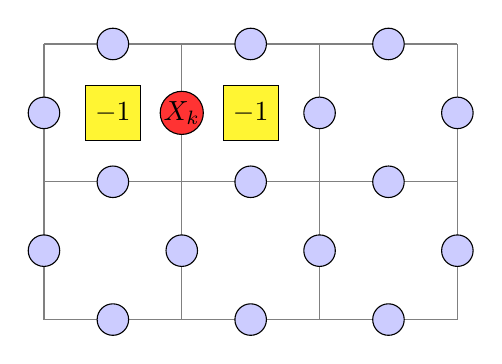
\begin{tikzpicture}[scale=1.75]
    \tikzstyle{dataq} = [circle, draw, fill=blue!20, inner sep=0pt, minimum size=4mm]
    \tikzstyle{defect} = [rectangle, draw, fill=yellow!80, inner sep=0pt, minimum size=7mm]
    \draw[step=1.0, gray, thin] (0,0) grid (3,2);
    \foreach \x in {0,...,3} \foreach \y in {0,...,2} {
        \ifnum\y<2 \node[dataq] at (\x, \y+0.5) {}; \fi
        \ifnum\x<3 \node[dataq] at (\x+0.5, \y) {}; \fi
    }
    \node[dataq, fill=red!80] (err) at (1, 1.5) {$X_k$}; 
    % \node at (0.88, 1.75) {$X_k$};
    \node[defect] (d1) at (0.5,1.5) {$-1$};
    \node[defect] (d2) at (1.5,1.5) {$-1$};
\end{tikzpicture}
\end{center}
\end{frame}

\begin{frame}
\frametitle{Error Chains}
\begin{itemize}
    \item A string of errors of the same type creates defects only at the \textbf{endpoints} of the chain.
    \item Example: A chain of three $Z$ errors ($Z_a, Z_b, Z_c$).
\end{itemize}
\begin{center}
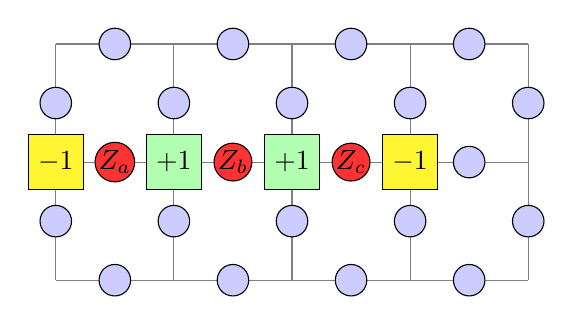
\begin{tikzpicture}[scale=1.5]
    \tikzstyle{dataq} = [circle, draw, fill=blue!20, inner sep=0pt, minimum size=4mm]
    \tikzstyle{vertexop} = [rectangle, draw, fill=green!30, inner sep=0pt, minimum size=7mm]
    \tikzstyle{defect} = [rectangle, draw, fill=yellow!80, inner sep=0pt, minimum size=7mm]
    \draw[step=1.0, gray, thin] (0,0) grid (4,2);
    \foreach \x in {0,...,4} \foreach \y in {0,...,2} {
        \ifnum\y<2 \node[dataq] at (\x, \y+0.5) {}; \fi
        \ifnum\x<4 \node[dataq] at (\x+0.5, \y) {}; \fi
    }
    \node[dataq, fill=red!80] at (0.5, 1) {$Z_a$};
    \node[dataq, fill=red!80] at (1.5, 1) {$Z_b$};
    \node[dataq, fill=red!80] at (2.5, 1) {$Z_c$};
    \node[defect] (v1) at (0,1) {$-1$};
    \node[vertexop] (v2) at (1,1) {$+1$};
    \node[vertexop] (v3) at (2,1) {$+1$};
    \node[defect] (v4) at (3,1) {$-1$};
\end{tikzpicture}
\end{center}
\end{frame}

\begin{frame}
\frametitle{Do $X$ Errors Form Chains?}
\begin{itemize}
    \item Motivation: Want to \href{https://gui.quantumcodes.io/2d}{show}\footnote{Thank you \href{https://github.com/panqec/panqec}{PanQEC} (Eric Huang \& Arthur Pesah)!} that $X$ errors also form chains.
\end{itemize}
\end{frame}

\begin{frame}
\frametitle{The Dual Lattice}
\begin{itemize}[<+->]
    \item The \textbf{Dual Lattice} is created by rotating all of the qubit edges by 90 degrees (orange dotted lines).
\begin{center}
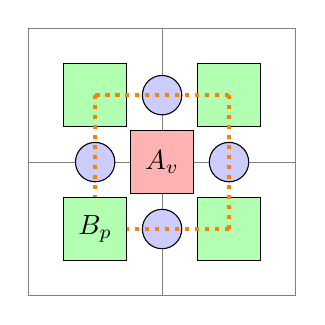
\begin{tikzpicture}[scale=1.7]
    \tikzstyle{dataq} = [circle, draw, fill=blue!20, inner sep=0pt, minimum size=5mm]
    \tikzstyle{vertexop} = [rectangle, draw, fill=red!30, inner sep=0pt, minimum size=8mm]
    \tikzstyle{plaqop} = [rectangle, draw, fill=green!30, inner sep=0pt, minimum size=8mm]
    \tikzstyle{dualvertex} = [circle, draw, fill=orange!50, inner sep=0pt, minimum size=4mm]

    % Primal Grid
    \draw[gray, thin] (0,0) grid (2,2);

    % Dual Grid
    \foreach \x in {0,...,1} \foreach \y in {0,...,1} {
        \node[plaqop] at (\x+0.5, \y+0.5) {};
    }

    % Data qubits
    \node[dataq] at (1, 0.5) {};
    \node[dataq] at (0.5, 1) {};
    \node[dataq] at (1.5, 1) {};
    \node[dataq] at (1, 1.5) {};

    \draw[orange, dotted, ultra thick] (0.5,0.5) -- (1.5,0.5);
    \draw[orange, dotted, ultra thick] (0.5,1.5) -- (1.5,1.5);
    \draw[orange, dotted, ultra thick] (0.5,0.5) -- (0.5,1.5);
    \draw[orange, dotted,ultra thick] (1.5,0.5) -- (1.5,1.5);

    \node[vertexop] (A11) at (1,1) {$A_v$};
    \node[plaqop] (B11) at (0.5,0.5) {$B_p$};
\end{tikzpicture}
\end{center}
    \item \textbf{Result}: Star Operators $\Leftrightarrow$ Plaquette Operators.
    \item An $X$ error chain on the dual lattice behaves like a $Z$ error chain on the primal lattice.
\end{itemize}
\end{frame}

\begin{frame}
    \frametitle{$X$ Error Chain on the Primal Lattice}
    \begin{center}
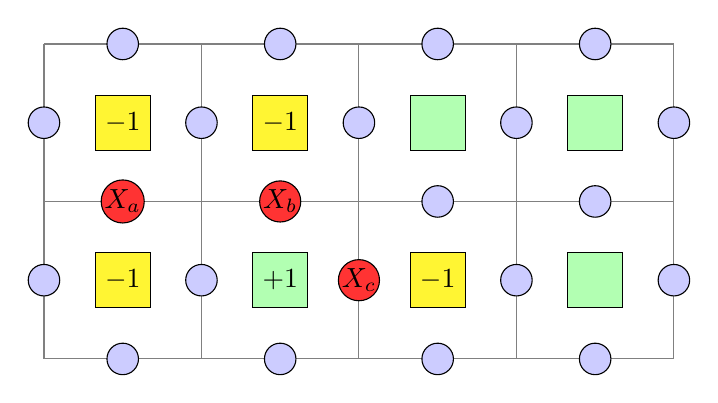
\begin{tikzpicture}[scale=2.0]
    \tikzstyle{dataq} = [circle, draw, fill=blue!20, inner sep=0pt, minimum size=4mm]
    \tikzstyle{plaqop} = [rectangle, draw, fill=green!30, inner sep=0pt, minimum size=7mm]
    \tikzstyle{defect} = [rectangle, draw, fill=yellow!80, inner sep=0pt, minimum size=7mm]

    % Grid
    \draw[step=1.0, gray, thin] (0,0) grid (4,2);

    % Data qubits
    \foreach \x in {0,...,4} \foreach \y in {0,...,2} {
        \ifnum\y<2 \node[dataq] at (\x, \y+0.5) {}; \fi
        \ifnum\x<4 \node[dataq] at (\x+0.5, \y) {}; \fi
    }
    % The error chain
    \node[dataq, fill=red!80] (err1) at (0.5, 1) {$X_a$};
    \node[dataq, fill=red!80] (err2) at (1.5, 1) {$X_b$};
    \node[dataq, fill=red!80] (err3) at (2, 0.5) {$X_c$};

    % Plaquettes
    \node[defect] (p1) at (0.5,0.5) {$-1$};
    \node[plaqop] (p2) at (1.5,0.5) {$+1$};
    \node[defect] (p3) at (2.5,0.5) {$-1$};
    \node[plaqop] (p4) at (3.5,0.5) {};
    \node[defect] (d1) at (0.5,1.5) {$-1$};
    \node[defect] (p5) at (1.5,1.5) {$-1$};
    \node[plaqop] (d2) at (2.5,1.5) {};
    \node[plaqop] (p6) at (3.5,1.5) {};

\end{tikzpicture}
\end{center}
\end{frame}

\begin{frame}
    \frametitle{$X$ Error Chain on the Dual Lattice}
    \begin{center}
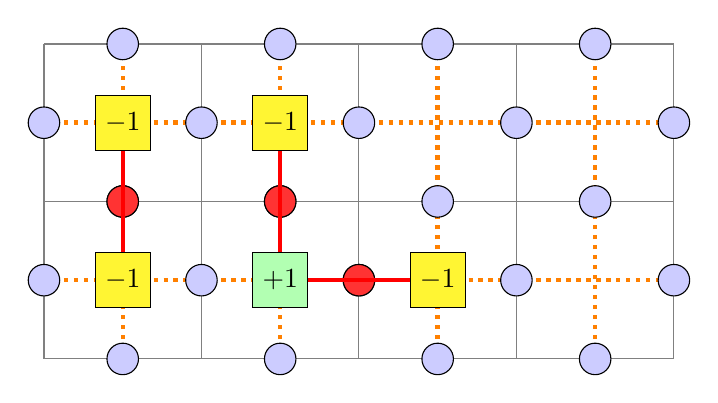
\begin{tikzpicture}[scale=2.0]
    \tikzstyle{dataq} = [circle, draw, fill=blue!20, inner sep=0pt, minimum size=4mm]
    \tikzstyle{plaqop} = [rectangle, draw, fill=green!30, inner sep=0pt, minimum size=7mm]
    \tikzstyle{defect} = [rectangle, draw, fill=yellow!80, inner sep=0pt, minimum size=7mm]
    \tikzstyle{dualvertex} = [circle, draw, fill=orange!50, inner sep=0pt, minimum size=4mm]

    % Primal Grid
    \draw[step=1.0, gray, thin] (0,0) grid (4,2);

    % Dual Grid
    % \foreach \x in {0,...,3} \foreach \y in {0,...,1} {
    %     \node[dualvertex] at (\x+0.5, \y+0.5) {};
    % }
    \foreach \x in {-0.5,...,2.5} \foreach \y in {0,...,1} {
        \draw[orange, dotted, ultra thick] (\x+0.5, \y+0.5) -- (\x+1.5, \y+0.5);
    }
    \foreach \x in {0,...,3} \foreach \y in {0,...,0} {
        \draw[orange, dotted, ultra thick] (\x+0.5, \y) -- (\x+0.5, \y+2);
    }

    % Data qubits
    \foreach \x in {0,...,4} \foreach \y in {0,...,2} {
        \ifnum\y<2 \node[dataq] at (\x, \y+0.5) {}; \fi
        \ifnum\x<4 \node[dataq] at (\x+0.5, \y) {}; \fi
    }
    
    % The error chain
    \node[dataq, fill=red!80] (err1) at (0.5, 1) {};
    \node[dataq, fill=red!80] (err2) at (1.5, 1) {};
    \node[dataq, fill=red!80] (err3) at (2, 0.5) {};

    % Draw the error path on the dual grid
    \draw[red, ultra thick] (0.5,0.5) -- (0.5,1.5);
    \draw[red, ultra thick] (1.5,0.5) -- (1.5,1.5);
    \draw[red, ultra thick] (1.5,0.5) -- (2.5,0.5);

    % Defects
    \node[defect] at (0.5,0.5) {$-1$};
    \node[defect] at (0.5,1.5) {$-1$};
    \node[plaqop] at (1.5,0.5) {$+1$};
    \node[defect] at (1.5,1.5) {$-1$};
    \node[defect] at (2.5,0.5) {$-1$};
\end{tikzpicture}
\end{center}
\end{frame}

\begin{frame}
\frametitle{Correcting Errors}
\begin{itemize}[<+->]
    \item The syndrome tells us the endpoints of an error chain.
    \item But which path did the error take? There are many possibilities.
    \item Let $E_{true}$ be the actual error. We make a guess, $E_{guess}$.
    \item We apply the correction for $E_{guess}$. The remaining error is $E_{guess} E_{true}$.
    \item This combined operation is a \textbf{loop} in the lattice.
    \begin{itemize}
        \item If the loop is a stabilizer, then $E_{guess} E_{true} |\psi_L\rangle = |\psi_L\rangle$.
        \item The correction works!
    \end{itemize}
\end{itemize}
\end{frame}

\begin{frame}
\frametitle{Logical Operators are Undetectable}
\begin{itemize}[<+->]
    \item What makes a loop a logical operator vs. a stabilizer?
    \item On a simple plane, all loops are stabilizers.
\begin{center}
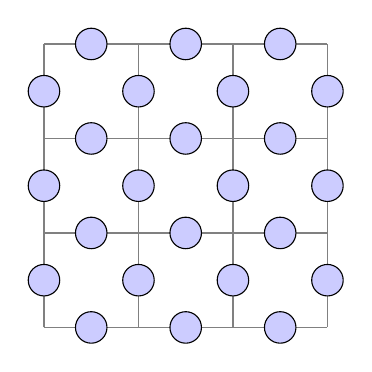
\begin{tikzpicture}[scale=1.2]
    \def\d{3}
    \tikzstyle{dataq} = [circle, draw, fill=blue!20, inner sep=0pt, minimum size=4mm]
    \draw[gray, thin] (0,0) grid (\d,\d);
    \foreach \y in {0,...,\d} {
        \foreach \x in {0,...,2} {
            \node[dataq] at (\x+0.5, \y) {};
        }
    }
    \foreach \x in {0,...,\d} {
        \foreach \y in {0,...,2} {
            \node[dataq] at (\x, \y+0.5) {};
        }
    }
\end{tikzpicture}
\end{center}
    \item To get a logical operator we need to create a non-trivial non-detectable operation.
    \item We can move the endpoints into each other, but this just creates stabilizer given the
    topology:
\end{itemize}
\end{frame}

\begin{frame}
\frametitle{Different Topologies}
\begin{itemize}
    \item To have logical operations we need a different topology:
\end{itemize}
\begin{columns}
\column{0.5\textwidth}
\begin{center}
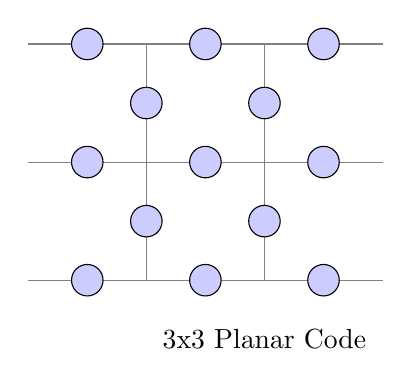
\begin{tikzpicture}[scale=1.5]
    \tikzstyle{dataq} = [circle, draw, fill=blue!20, inner sep=0pt, minimum size=4mm]

    % Draw grid lines
    
    % Draw all horizontal lines (from y=0 to y=4)
    \foreach \y in {0,...,2} {
        \draw[gray, thin] (0,\y) -- (3,\y);
    }
    
    % Draw only the inner vertical lines (from x=1 to x=3)
    % This skips the outer lines at x=0 and x=4
    \foreach \x in {1,...,2} {
        \draw[gray, thin] (\x,0) -- (\x,2);
    }

    % Horizontal data qubits
    \foreach \y in {0,...,2} {
        \foreach \x in {0,...,2} {
            \node[dataq] at (\x+0.5, \y) {};
        }
    }
    % Vertical data qubits (not on left/right boundaries)
    \foreach \y in {0,...,1} {
        \foreach \x in {1,...,2} {
            \node[dataq] at (\x, \y+0.5) {};
        }
    }
    \node at (2, -0.5) {3x3 Planar Code};
\end{tikzpicture}
\end{center}
\column{0.5\textwidth}
\begin{center}
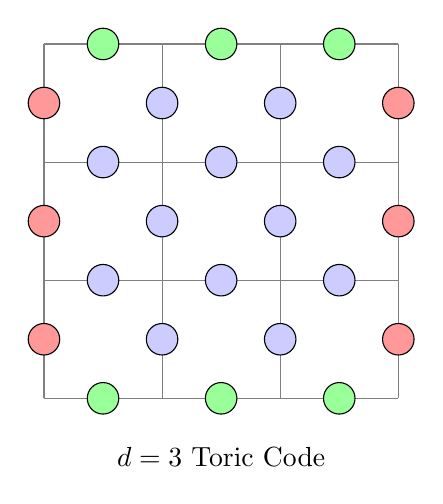
\begin{tikzpicture}[scale=1.5]
    \def\d{3}
    
    % --- DEFINE STYLES ---
    % Style for bulk qubits
    \tikzstyle{dataq} = [circle, draw, fill=blue!20, inner sep=0pt, minimum size=4mm]
    % Style for horizontal (top/bottom) boundary qubits
    \tikzstyle{h_boundary_q} = [dataq, fill=green!40]
    % Style for vertical (left/right) boundary qubits
    \tikzstyle{v_boundary_q} = [dataq, fill=red!40]

    % Draw grid
    \draw[gray, thin] (0,0) grid (\d,\d);

    % --- DRAW QUBITS WITH CONDITIONAL STYLING ---

    \foreach \y in {0,...,\d} {
        \foreach \x in {0,...,2} {
            % Check if y is on the top or bottom boundary
            \ifnum\y=0 \def\style{h_boundary_q}
            \else
                \ifnum\y=\d \def\style{h_boundary_q}
                \else \def\style{dataq}
                \fi
            \fi
            % Draw the node with the chosen style
            \node[\style] at (\x+0.5, \y) {};
        }
    }
    
    \foreach \x in {0,...,\d} {
        \foreach \y in {0,...,2} {
            % Check if x is on the left or right boundary
            \ifnum\x=0 \def\style{v_boundary_q}
            \else
                \ifnum\x=\d \def\style{v_boundary_q}
                \else \def\style{dataq}
                \fi
            \fi
            % Draw the node with the chosen style
            \node[\style] at (\x, \y+0.5) {};
        }
    }

    % Identification labels
    \node at (\d/2, -0.5) {$d=3$ Toric Code};
\end{tikzpicture}
\end{center}
\end{columns}
\end{frame}

\begin{frame}
\frametitle{Logical Operators on the Torus}
\begin{itemize}[<+->]
    \item On a torus, there are non-trivial loops that cannot be shrunk to a point.
    \item These correspond to logical operators, the Toric Code has four of them.
    \item \textbf{Logical $\overline{Z}$:} A string of $Z$ operators wrapping around the torus (both directions).
    \item \textbf{Logical $\overline{X}$:} A string of $X$ operators wrapping around the torus (both directions).
\end{itemize}
\begin{columns}
\column{0.5\textwidth}
\begin{center}
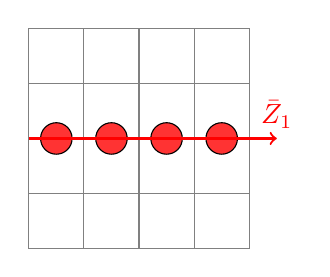
\begin{tikzpicture}[scale=0.7]
    \tikzstyle{dataq} = [circle, draw, fill=blue!20, inner sep=0pt, minimum size=4mm]
    \draw[step=1.0, gray, thin] (0,0) grid (4,4);
    \foreach \x in {0,...,3} {
        \node[dataq, fill=red!80] at (\x+0.5, 2) {};
    }
    \draw[red, thick, ->] (0, 2) -- (4.5, 2) node[above] {$\bar{Z}_1$};
\end{tikzpicture}
\end{center}
\column{0.5\textwidth}
\begin{center}
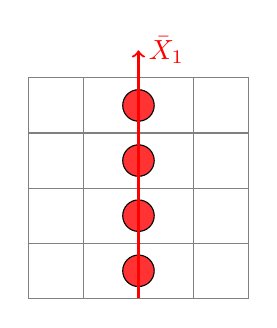
\begin{tikzpicture}[scale=0.7]
    \tikzstyle{dataq} = [circle, draw, fill=blue!20, inner sep=0pt, minimum size=4mm]
    \draw[step=1.0, gray, thin] (0,0) grid (4,4);
    \foreach \y in {0,...,3} {
        \node[dataq, fill=red!80] at (2, \y+0.5) {};
    }
    \draw[red, thick, ->] (2, 0) -- (2, 4.5) node[right] {$\bar{X}_1$};
\end{tikzpicture}
\end{center}
\end{columns}
\end{frame}

\begin{frame}
\frametitle{Toric Code Properties}
\begin{columns}
\column{0.5\textwidth}
\begin{itemize}[<+->]
    \item For an $L \times L$ toric code, we have $2L^2$ data qubits.
    % QUESTION FOR AUDIENCE
    % How many vertex generators?
    \item There are $L^2$ star generators and $L^2$ plaquette generators.
    \item Total \textbf{independent} stabilizers: $2L^2 - 2$.
    \item Number of logical qubits $k = n - (\text{\# of generators}) = 2$.
    \item The \textbf{code distance} $d$ is the length of the shortest logical operator, which is $L$.
    \item So, the toric code is a $[[2L^2, 2, L]]$ code; correcting up to $t = \lfloor(L-1)/2\rfloor$ errors.
\end{itemize}
\column{0.5\textwidth}
\begin{center}
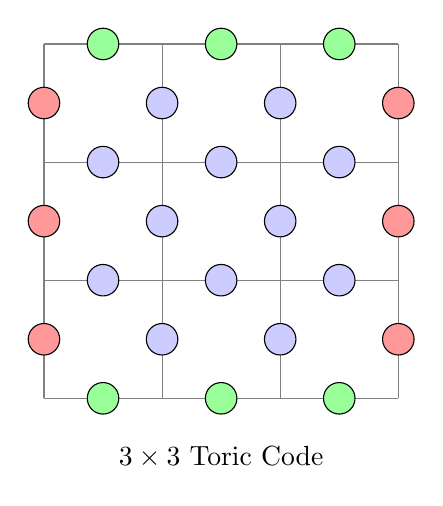
\begin{tikzpicture}[scale=1.5]
    \def\d{3}
    
    % --- DEFINE STYLES ---
    % Style for bulk qubits
    \tikzstyle{dataq} = [circle, draw, fill=blue!20, inner sep=0pt, minimum size=4mm]
    % Style for horizontal (top/bottom) boundary qubits
    \tikzstyle{h_boundary_q} = [dataq, fill=green!40]
    % Style for vertical (left/right) boundary qubits
    \tikzstyle{v_boundary_q} = [dataq, fill=red!40]

    % Draw grid
    \draw[gray, thin] (0,0) grid (\d,\d);

    % --- DRAW QUBITS WITH CONDITIONAL STYLING ---

    \foreach \y in {0,...,\d} {
        \foreach \x in {0,...,2} {
            % Check if y is on the top or bottom boundary
            \ifnum\y=0 \def\style{h_boundary_q}
            \else
                \ifnum\y=\d \def\style{h_boundary_q}
                \else \def\style{dataq}
                \fi
            \fi
            % Draw the node with the chosen style
            \node[\style] at (\x+0.5, \y) {};
        }
    }
    
    \foreach \x in {0,...,\d} {
        \foreach \y in {0,...,2} {
            % Check if x is on the left or right boundary
            \ifnum\x=0 \def\style{v_boundary_q}
            \else
                \ifnum\x=\d \def\style{v_boundary_q}
                \else \def\style{dataq}
                \fi
            \fi
            % Draw the node with the chosen style
            \node[\style] at (\x, \y+0.5) {};
        }
    }

    % Identification labels
    \node at (\d/2, -0.5) {$3\times 3$ Toric Code};
\end{tikzpicture}
\end{center}
\end{columns}
\end{frame}

\begin{frame}
\frametitle{Toric Code: Decoding}
\begin{itemize}[<+->]
    \item Decode surface code errors by finding \emph{most likely} error path to explain observed detectors.
    \item Many approaches:
    \begin{itemize}
        \item Minimum Weight Perfect Matching.
        \item Belief Propagation + Ordered Statistics.
    \end{itemize}
    \item Tradeoffs between correctness and runtime.
    \item \href{file:///Users/dandragona/Downloads/index.html}{Tesseract Decoder}
\end{itemize}
\end{frame}

\end{document}
